%!TEX root = ../main.tex

Dans ce troisième chapitre, toutes les connaissances acquises durant l'étude seront mises en œuvre pour atteindre
une machine qui est supposée être sécurisée. %vérifié

La démarche que nous allons suivre est la suivante : 
\begin{itemize}
    \item Nous allons développer un Malware hybride constitué d'un virus et d'un backdoor;
    \item Le Malware sera introduit manuellement dans une machine vulnérable qui est en communication continue
        avec la machine sécurisée;
    \item Ensuite, le Malware se propagera jusqu'à la machine sécurisée sans déclencher d'alerte;
    \item Finalement, un accès total est obtenu sur la machine sécurisée par le biais du backdoor.
\end{itemize}%vérifié

Le succès de cette opération démontrera indéniablement que la sécurité d'une machine dépend toujours
de la sécurité des machines avec lesquelles elle interagit.%vérifié

\newpage

\section{Préparation de l'environnement} \label{preparation_environnement}
Dans cette section, l'environnement et les outils nécessaires pour le bon fonctionnement du projet seront installés
et préparés correctement. Il y en a au totale trois machines différentes : une machine d'attaque, une machine vulnérable,
et finalement une machine sécurisée. %vérifié

    \subsubsection{La machine d'attaque} 
    Cette machine sera équipée du système d'exploitation \emph{Kali Linux \cite{linux} Rolling} 
    (\autoref{kali_linux}), le 
    leader des systèmes de test d'intrusions. Après le téléchargement de l'image
    ISO depuis le site officiel de Kali, et l'installation de l'image sur
    une machine virtuelle, une mise à jour complète du système est faite par le biais de cette commande : 
    ``\texttt{sudo apt-get update \&\& sudo apt-get upgrade}''  %vérifié

    \begin{figure}[h!]
        \centering
        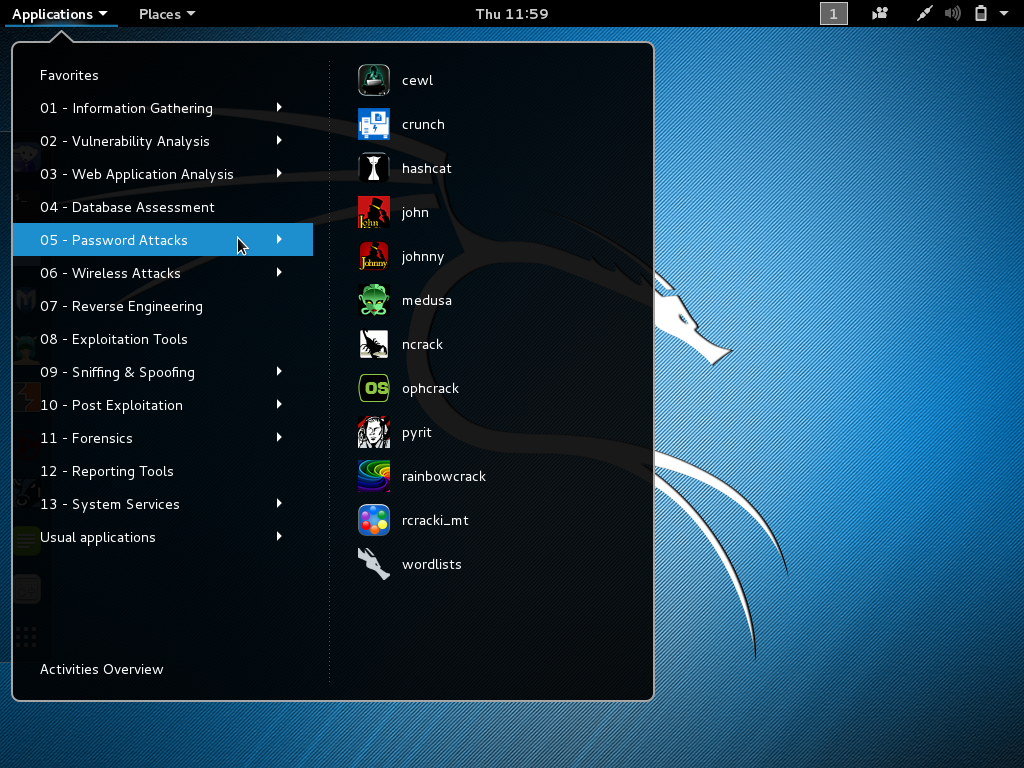
\includegraphics[width=\linewidth]{images/kali_linux.png}
        \caption{Kali Linux}
        \label{kali_linux}
    \end{figure}

    \subsubsection{La machine vulnérable} \label{machine_vulnerable} 
    Cette machine sera équipée d'une version \emph{Windows 7}  
    dotée d'un service vulnérable et d'un pare-feu désactivé. Le service vulnérable installé sur cette 
    machine est un service \emph{FTP} manipulé par le programme \emph{KONICA MINOLTA FTP Utility} 
    (\autoref{la_machine_vulnerable}). %vérifié
    \begin{figure}[h!]
        \centering
        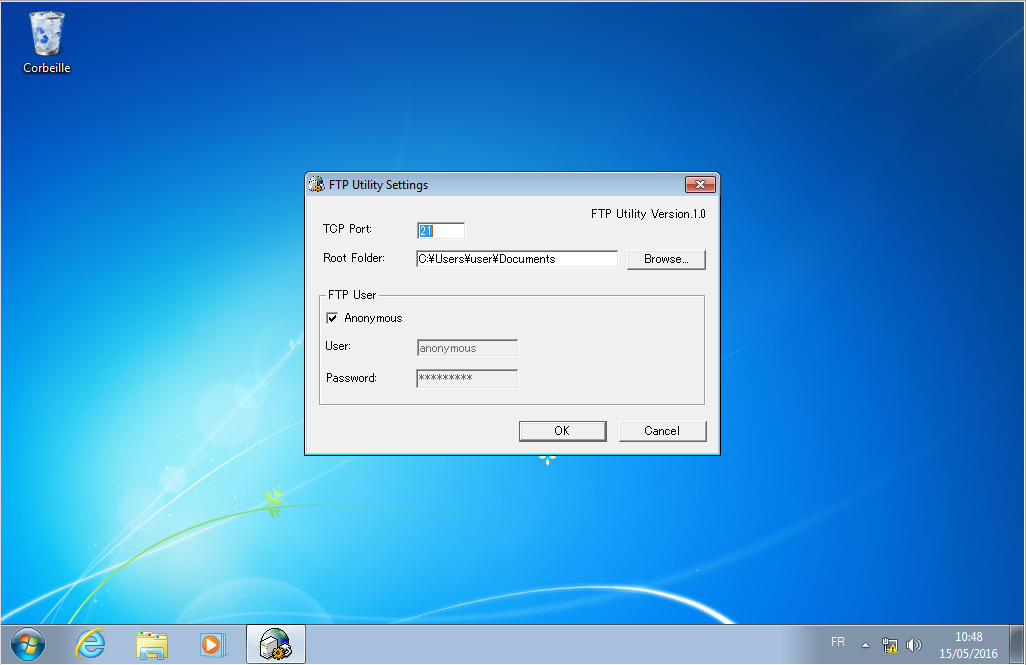
\includegraphics[scale=0.3]{images/Windows_7_2.png}
        \caption{La machine vulnérable}
        \label{la_machine_vulnerable}
    \end{figure}

    \subsubsection{La machine sécurisée} 
    Cette machine sera équipée de \emph{Windows 7} avec un pare-feu fonctionnel et la dernière version de l'anti-virus 
    \emph{Kaspersky} dont la base de données a été mise à jour (\autoref{mise_a_jour_kaspersky}). %vérifié

    \begin{figure}[!h]
        \centering
        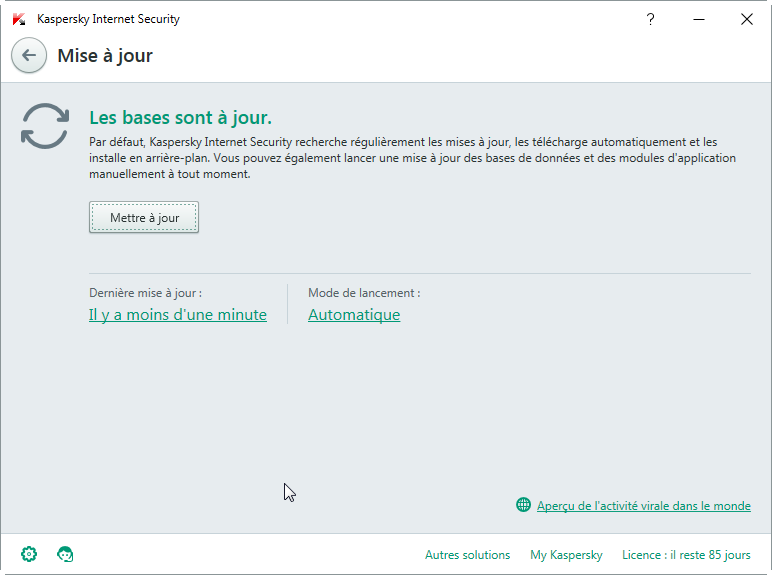
\includegraphics[width=\linewidth]{images/mise_a_jour_kaspersky.png}
        \caption{Mise à jours Kaspersky}
        \label{mise_a_jour_kaspersky}
    \end{figure}

\subsection{Réseau}
    Les trois machines seront dans le réseau dont l'adresse est \emph{172.16.178.0/24}, le tableau ci-dessous résume les adresses affectées a chaque machine de l'environnement
\begin{table}[h] % Le 'h' pour que la tableau soit dans la position qu'on vient d'indiquer.

    \begin{center} % Pour centrer notre tableau dans le document.

    \begin{tabular}{|c|c|c|}
    \hline
    Les machines & Adresse IP & Masque \\
    \hline
    La machine d'attaque & 172.16.178.1 & 255.255.255.0 \\
    \hline
    La machine vulnérable & 172.16.178.129 & 255.255.255.0 \\
    \hline
    La machine sécurisé & 172.16.178.130 & 255.255.255.0 \\
    \hline
    \end{tabular}

    \caption{Les adresses des machines} % On donne une légende à notre tableau
    \label{adresses_machines} % On marque notre tableau pour qu'on puisse utiliser sa référence plus tard (c'est facultatif).

    \end{center}
\end{table}

\section{Développement}
    \subsection{Backdoor}
    Dans cette section, deux programmes seront développés : un programme qui s'exécutera sur la machine victime
    qui représentera le backdoor , et un autre qui s'exécutera sur la machine assaillante. %vérifié
        \subsubsection{Côté victime}
        Le langage utilisé pour développer ce programme est le langage \emph{C} \cite{C}.

        Pour établir la connexion avec le backdoor, nous avons utilisé une technique appelée \emph{reverse connection}. 
        En utilisant cette dernière, au lieu que le backdoor ouvre un port et attend que nous nous  connectons à ce 
        port pour communiquer avec lui, il va plutôt essayer d'établir une connexion vers nous. 

        Cela permettra d'éviter la demande
        d'ouverture d'un port au pare-feu et l'éveil des soupçons de l'administrateur de la machine ; 
        par conséquent, le backdoor sera encore plus difficile à détecter.%vérifié

        En ce qui concerne le fonctionnement du backdoor, celui-ci a été simplifié le plus possible au vu de réduire 
        sa taille et pour que l'infection (\autoref{virus_infecteur}) passe inaperçue, et lui donné plus de 
        chance d'échapper aux anti-virus. 
        Malgré que les fonctionnalités ont été limitées, nous avons donné la capacité à notre backdoor 
        d'évoluer et d’intégrer plus de fonctionnalités.
        Les fonctionnalités actuelles se résument à ce qui suit : 

        \begin{description}
            \item[Accès sécurisé :] Dés le moment où le backdoor établi la connexion, un mot de passe est
                demandé par ce dernier (\autoref{backdoor_password}); si le mot de passe renseigné est correct, 
                alors l'accès est accordé, sinon la connexion s'arrête immédiatement. %vérifié

                \begin{figure}[h!]
                    \centering
                    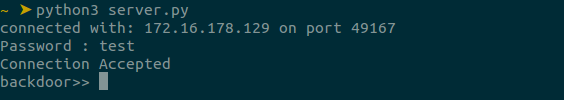
\includegraphics[width=0.9\linewidth]{images/backdoor_password.png}
                    \caption{Demande de mot de passe}
                    \label{backdoor_password}
                \end{figure}

                Pour éviter que le mot de passe soit découvert en \emph{désassemblant} l'exécutable du backdoor,
                une version hachée est conservée et utilisée pour valider le mot de passe fournie au moment de la 
                connexion. %vérifié

            \item[Accès à l'invite de commande :] Avec cette fonctionnalité, 
                chaque message envoyé par nous est redirigé vers la ligne 
                de commande de Windows, et la réponse de cette dernière est alors renvoyée.
                \begin{figure}[h!]
                    \centering
                    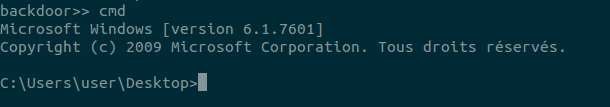
\includegraphics[width=0.9\linewidth]{images/backdoor_cmd.png}
                    \caption{Invite de commande}
                    \label{backdoor_cmd}
                \end{figure}

            \item[Envoi et réception de fichiers :] Cette fonctionnalité nous permet d'échanger des fichiers 
                avec le backdoor. Ainsi, nous pourrons envoyer et recevoir des fichiers depuis la machine victime.%vérifié

            \item[Mise à jour:] Cette fonctionnalité nous permet d'étendre les fonctionnalités du
                backdoor, en le remplaçant par un autre plus sophistiqué et plus complet. 
        \end{description}

        En ce qui concerne le lancement du backdoor ce dernier sera lancé périodiquement par le virus, pour 
        diminuer les chances qu'une inspection des communications réseau puisse découvrir sa présence.%vérifié

        \subsubsection{Côté assaillant}
        L'utilisation d'un logiciel de communication réseau (comme netcat \autoref{netcat}) 
        est amplement suffisant pour communiquer avec 
        le backdoor, mais pour exploiter toutes les fonctionnalités de ce dernier, il est indispensable 
        de développer un programme qui permettra de communiquer avec. %vérifié

        Ce programme qu'on a développé avec le langage \emph{python} \cite{python}, écoutera sur un port donné, 
        et attendra la connexion du backdoor. Une fois cette dernière établie, ce programme permettra d'envoyer 
        des commandes, et de recevoir leurs réponses.

        \subsubsection{Backdoor amélioré}
        Ce backdoor, en plus d'intégrer toutes les fonctionnalités de l'ancien, il établit une connexion 
        cryptée basée sur le protocole \emph{TLS}\footnote{Le \emph{TLS} (\emph{Transport Layer Security})
        est un protocole de sécurisation des communications réseau.}.%vérifié

        Pour illustrer cela, le logiciel \emph{Wireshark}\footnote{\emph{Wireshark} est un analyseur de 
        paquets réseau multi-plateforme supportant plusieurs centaines de protocoles. Il permet d’examiner les 
        données qui transitent sur le réseau, et par conséquence voir le contenu des paquets en direct et en détails.} 
        a été utilisé pour montrer la différence entre la communication 
        en claire utilisée par le premier backdoor (\autoref{communication_claire})
        , et la communication cryptée utilisée par le backdoor amélioré (\autoref{communication_cryptee}).

        Nous avons développer ce backdoor améliorer avec le langage \emph{python}. 
        Ensuite, nous avons utilisé un 
        compilateur nommé \emph{PyInstaller}. Ce dernier permet de générer un exécutable autonome qui peut être exécuté
        sur n'importe quelle machine Windows.

        \begin{figure}[H]
            \centering
            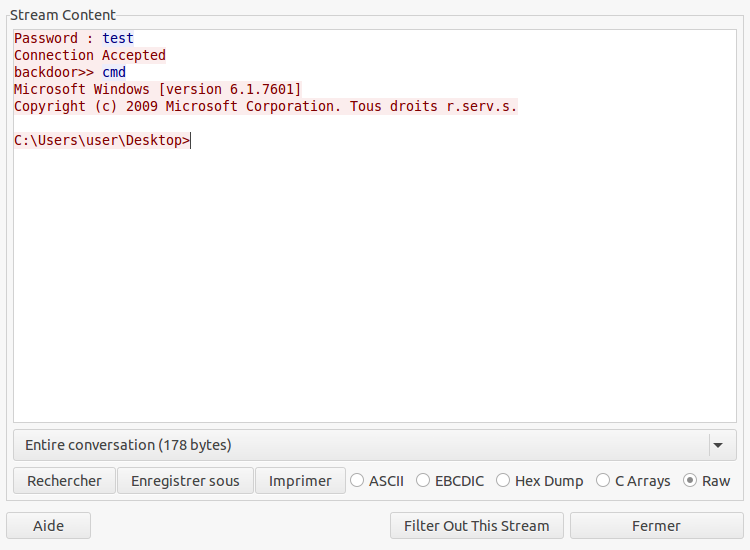
\includegraphics[width=0.8\linewidth, height=250pt]{images/communication_claire.png}
            \caption{Communication en claire}
            \label{communication_claire}
        \end{figure}

\newpage

        \begin{figure}[H]
            \centering
            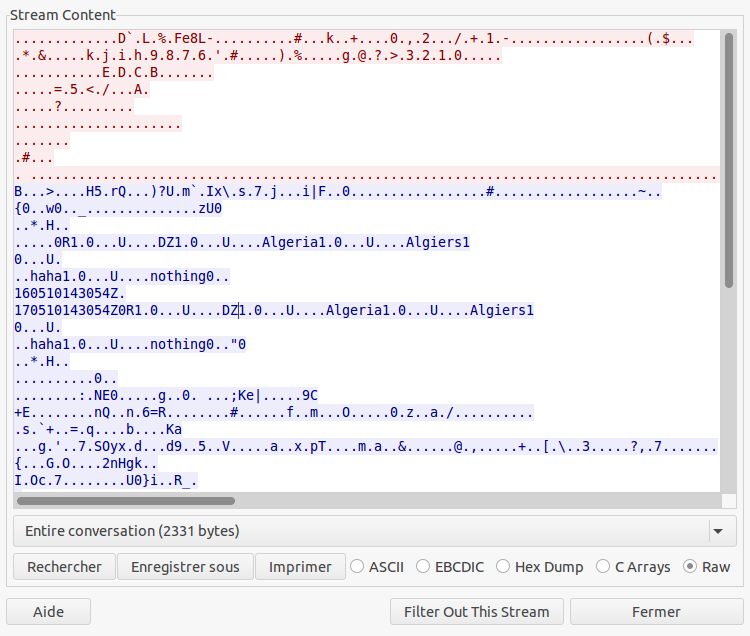
\includegraphics[width=0.8\linewidth, height=250pt]{images/communication_cryptee.png}
            \caption{Communication crypté avec le protocole TLS}
            \label{communication_cryptee}
        \end{figure}


    \subsection{Virus} \label{virus_infecteur}
    La méthode d’infection que nous allons utiliser est : l’injection de code dans un exécutable par \emph{Ajout}
    dont une définition claire a été abordée dans la \autoref{infeciton_ajout}.

    Cette technique se base sur la manipulation de la structure PE (une définition détaillée a été donnée dans le 
    \autoref{pe_header}), nous avons donc inclus la bibliothèque \emph{Windows.h} qui contient les 
    structures et fonctions nécessaires.

    Le code que nous avons développé avec le langage de programmation C se divise en deux fonctions primordiales :
    \begin{description}
        \item[WinMain :] Cette fonction est la fonction principale, car dans un premier temps son rôle est de créer 
        un espace mémoire et de copier tout l'exécutable du Virus dedans, puis de créer un second espace mémoire 
        pour  stocker le BackDoor, et enfin, elle cible un exécutable après avoir vérifier sa compatibilité avec Windows.

        Dans un deuxième temps, elle ouvre ce dernier et récupère sa structure PE. Après des calculs précis, 
        elle stocke dans une variable le \emph{Point d'Entrer} Original appelé \emph{OEP} et ajoute à la fin 
        de ce fichier deux nouveaux segments, à savoir :

        Le segment VIRUS qui est devisé en deux parties, la première partie contient le code de la fonction NEP\_VIRUS 
        qui est définie dans le corps de l'exécutable du Virus, ce code sera le nouveau point d'entré de l'exécutable 
        infecté, après cela viens la seconde partie contenant le corps du Virus ayant été stocker dans un espace mémoire.
       
        Le segment BackDoor qui contient le BackDoor ayant été stocké dans le second espace mémoire.

        De ce fait, cette fonction crypte le segment du BackDoor, et la deuxième partie du segment virus avec une clé prédéfinie.

        A la fin, elle change le point d’entré et le fait pointer vers la première partie du premier segment 
        (\autoref{entrypoint_changement}).
        La fonction modifie aussi le \emph{loader flags}\footnote{\emph{loader flags} est un flag obsolète non
        utiliser par Windows comme expliqué dans ce lien 
        \url{https://msdn.microsoft.com/en-us/library/windows/desktop/ms680339(v=vs.85).aspx}.} et y place notre 
        flag d'infection. En dernier, une correction du \emph{Checksum} sera faite.

        \item[NEP\_VIRUS :] Cette fonction sera le nouveau point d’enté de chaque exécutable infecté, elle s'exécutera 
            toujours en premier puis elle donnera la main au code original, en passant par trois étapes clé :

            Premièrement, puisque cette fonction n'a pas été compilé avec l’exécutable hôte, elle ne connaît pas les 
            adresses des fonctions qu'elle va utilisée, donc une récupération de l’adresse de la bibliothèque 
            \emph{Kernel32} chargée avec l’exécutable hôte est primordiale et suffisante pour trouver et stocker les
            adresses des fonctions nécessaires au bon fonctionnement du code malveillant.

            Deuxièmement, elle chargera l’adresse du segment  Backdoor et l'adresse de début du corps du Virus stocker 
            dans le premier segment, créera deux emplacements mémoire et les copiera dedans, puis elle les décrypte.

            Et enfin, elle créera deux fichiers exécutables dans le dossier ``temp'', un, contenant le corps Virus et 
            l’autre le Backdoor et les exécutera. En dernier, un appel vers le point d’entré original sera fait
            pour redonner la main à l'exécutable hôte, ce qui permettra d'éviter l'éveil des soupçons.
    \end{description}

\newpage

    \begin{figure}[H]
        \centering
        \begin{subfigure}{0.9\textwidth}
            \centering
            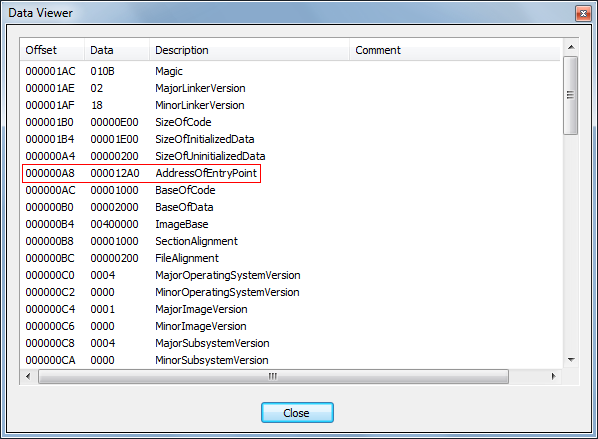
\includegraphics[width=\textwidth]{images/entrypoint_avant.png}
            \caption{Point d'entrée avant infection}
            \label{entrypoint_avant}
        \end{subfigure}
        \hfill
        \begin{subfigure}{0.9\textwidth}
            \centering
            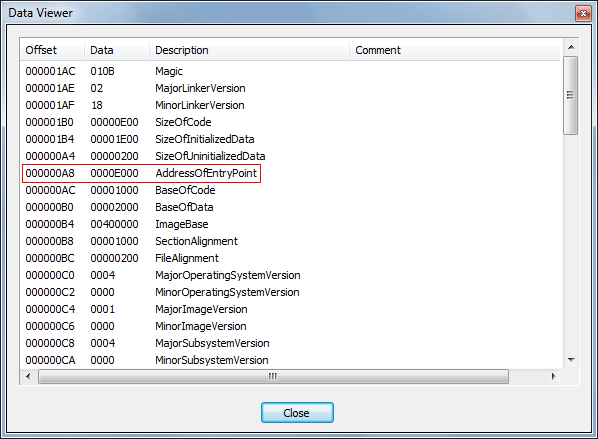
\includegraphics[width=\textwidth]{images/entrypoint_after.png}
            \caption{Point d'entrée après infection}
            \label{entrypoint_apres}
        \end{subfigure}
        \hfill
        \caption{Changement du point d'entrée de l'exécutable}
        \label{entrypoint_changement}
    \end{figure}

    Nous citerons aussi que ce Virus infecte les fichiers exécutables des clés USB connectées à la machine.
    La particularité majeure de notre Virus est qu’il utilise des API natives et qu’il ne peut pas être 
    débogué.

\section{Exploitation} \label{exploitation}
Cette section sera consacrée à l'exploitation de la machine vulnérable et l'obtention d'un accès à distance
sur cette dernière. Nous commencerons par une brève présentation des outils utilisés pour une meilleure compréhension
de cette section.
    \subsection{Présentation des outils}
    \begin{description}
        \item[netcat :] \label{netcat}
            C'est un outil utilisé en ligne de commande, et qui permet l'ouverture des connexions
            réseau, que ce soit \emph{TCP} \cite{reseau} ou \emph{UDP} \cite{reseau}. En raison de sa polyvalence,
            il est aussi appelé le \emph{couteau suisse} du réseau.
            Pour se connecter à un serveur sur un port donné, il faut donner à \emph{netcat} deux paramètres qui sont, 
            l'adresse du serveur et le port qu'utilise le serveur. Exemple :
            \begin{lstlisting}[language=bash] 
            $ netcat www.google.com 80
            \end{lstlisting}

            Dans le côté serveur, pour mettre netcat en écoute sur un port, il faut préciser deux options qui sont 
            `\emph{-l}' pour dire à netcat d'écouter, et `\emph{-p \ul{port}}' pour préciser le port d'écoute.
            Exemple :
            \begin{lstlisting}
            # netcat -l -p 80   
            \end{lstlisting}

        \item[Metasploit :] C'est un \emph{Framework} de test de pénétrations \emph{open source} utilisé pour 
            tester la robustesse des machines en matière de sécurité. Il est composé essentiellement de charges 
            et d'exploits. 

        \item[msfvenom :] \label{msfvenom} C'est un générateur et encodeurs de charges. Il est utile pour une 
            utilisation plus manuelle des charges, car il permet de générer ces dernières dans plusieurs formats 
            (des exécutables, pour un script python \ldots{}). 

            Plusieurs paramètres sont à utiliser pour obtenir des charges plus performantes. Parmi ces options, on y
            trouve :
            \begin{description}
                \item[-a \ul{architecture} :] L'architecture du système dont la charge est destinée
                    (x86 ou x64).
                \item[--plateform \ul{plateforme} :] Le système attaqué (Windows, Mac, Linux, Android
                \ldots{}).
                \item[-p \ul{charge} \ul{options\_de\_la\_charge}:] La charge et les options utilisées 
                    pour générer celle-ci.
                \item[-e \ul{encodage} :] L'encodage utilisé pour générer la charge.
                \item[-b \ul{mauvais\_octets} :] Les octets à éviter pendant la génération de la charge.
                \item[-f \ul{format} :] Format de la charge (exécutable, python, perl \ldots{}).
            \end{description}

        \item[meterpreter :] \label{meterpreter}C'est une charge avancée et extensible développer par les développeurs 
            de \emph{Metasploit}. Elle est utilisée par ce dernier pour donner un accès plus étendu et plus 
            complet à une machine exploitable. 
    \end{description}

    \subsection{Le programme vulnérable}
    Le programme vulnérable que nous allons exploiter se nomme \emph{Konica Minolta FTP Utility} 
    (\autoref{konica_minolta}). 
    C'est un programme gratuit utilisé pour la réception de données envoyées depuis des appareils compatible en 
    utilisant le scan vers \emph{FTP}\footnote{Le \emph{FTP} est un protocole destiné
    à l'échange informatique des fichiers sur un réseau.}. Le programme permet à l'utilisateur de recevoir des données 
    depuis des produits multifonctionnels, il authentifie le nom d'utilisateur et le mot de passe et sauvegarde les
    données reçues dans le dossier de réception \cite{konica_minolta}. Plus de \emph{vingt mille} exemplaires de ce 
    programme ont été télécharger depuis son apparition (\autoref{konica_minolta_site}). %vérifié

    \begin{figure}[h]
        \centering
        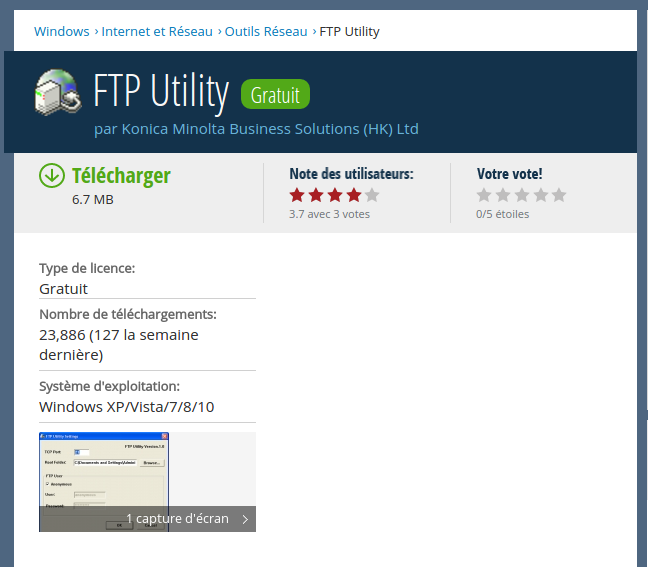
\includegraphics[width=0.8\linewidth]{images/konica_minolta.png}
        \caption{Konica Minolta FTP Utility}
        \label{konica_minolta}
    \end{figure}
    
    \begin{figure}[h]
        \centering
        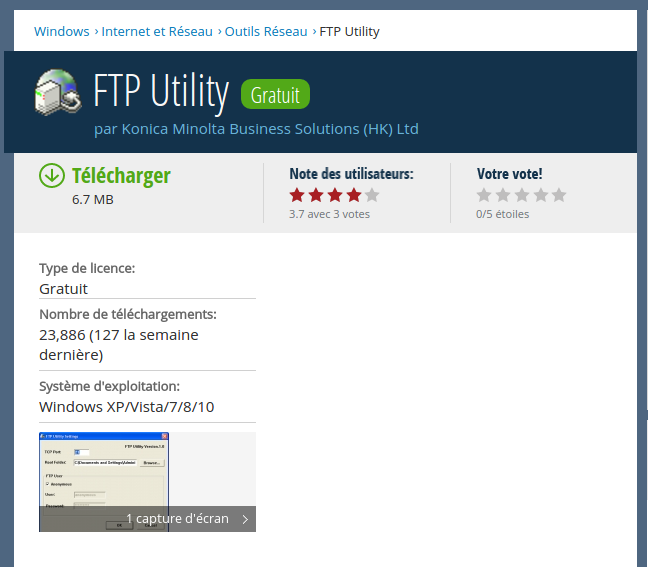
\includegraphics[width=0.8\linewidth]{images/konica_minolta_site.png}
        \caption{Site de Konica Minolta FTP Utility}
        \label{konica_minolta_site}
    \end{figure}

    La version vulnérable, qui est la \emph{version 1.0} 
    (la dernière jusqu'à maintenant), peut-être obtenue depuis ce lien \\\url{https://www.exploit-db.com/apps/6388a2ae7dd2965225b3c8fad62f2b3b-ftpu_10.zip}. %vérifié
     
    La vulnérabilité découverte dans ce programme est un débordement de tampon (\autoref{buffer_overflow}). 
    Elle a été publiée le 21 janvier 2016 sur le site d'\emph{Exploit Database} 
    \footnote{\emph{Exploit Database} est un site qui se charge d'archiver les exploits publics et les 
    logiciels vulnérables correspondants. Ce site dont le lien est \url{www.exploit-db.com} est développé 
    par les testeurs d'intrusions et les chercheurs de vulnérabilités.} par un contributeur surnommé \emph{TOMIWA}.
    %vérifié

    \subsection{L'exploit}
    Le script qui permet d'exploiter cette vulnérabilité peut être récupéré depuis ce lien 
    \url{https://www.exploit-db.com/exploits/39215/}. Ce script \emph{python} \cite{python} se divise en deux parties :
    \begin{description}
        \item[Exploit :] Cette partie du script permet en quelque sorte de préparer le programme vulnérable à 
            recevoir le code malveillant pour l'exécution. Cette partie n'est pas à modifier, car elle a été développée
            après une étude approfondie du programme vulnérable.

        \item[Charge :] Cette partie du script représente le code qui sera exécuté sur l'application vulnérable. 
            Cette partie peut être remplacée par la charge désirée par l'attaquant.
    \end{description}

    Le script va se connecter à la machine victime sur le port 21 (\autoref{execution_script_exploitation}). 
    La charge qu'utilise le script va ordonner à la machine qu'elle donne un reverse shell en se reconnectant à 
    la machine de l'attaquant sur le port 4444. Pour intercepter ce reverse shell et pouvoir communiquer avec
    la machine victime, il faut ordonner à netcat d'écouter sur le port 4444 (\autoref{obtention_reverse_shell}).

    \begin{figure}[h!]
        \centering
        \begin{subfigure}{0.9\textwidth}
            \centering
            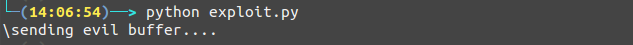
\includegraphics[width=\textwidth]{images/exploit_python.png}
            \caption{Exécution du script d'exploitation}
            \label{execution_script_exploitation}
        \end{subfigure}
        \hfill
        \begin{subfigure}{0.9\textwidth}
            \centering
            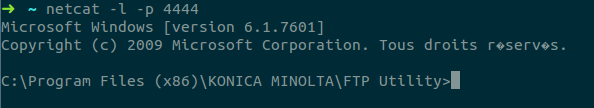
\includegraphics[width=\textwidth]{images/reverse_shell.png}
            \caption{Obtention du reverse shell}
            \label{obtention_reverse_shell}
        \end{subfigure}
        \hfill
        \caption{Exploitation avec la charge d'origine}
        \label{exploitation_avec_charge_origine}
    \end{figure}

    La charge par défaut de ce script est une charge un petit peu limitée, donc nous allons nous servir 
    de \emph{msfvenom} pour générer la charge \emph{meterpreter} (\autoref{generation_charge}) et l'utiliser 
    dans le script d'exploitation.
    \begin{figure}[h]
        \centering
        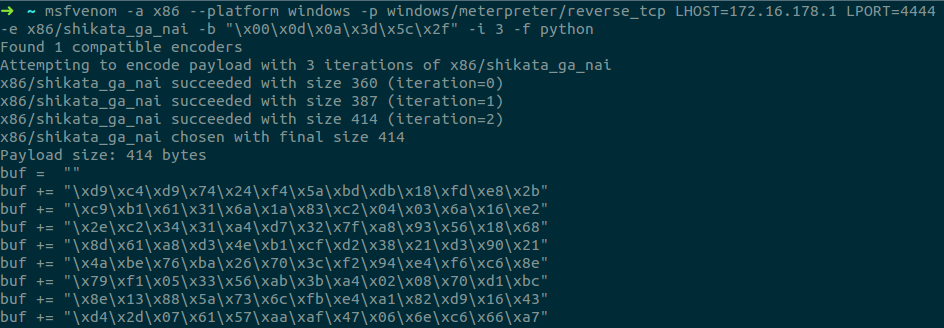
\includegraphics[width=\linewidth]{images/msfvenom.png}
        \caption{Génération de la charge}
        \label{generation_charge}
    \end{figure}

    \subsection{Obtention d'accès}
    Pour la charge appliquée précédemment, il a suffit d'utiliser netcat pour intercepter la connexion et communiquer
    avec la machine victime. Mais meterpreter exige des techniques plus poussées pour pouvoir faire cela, 
    donc nous allons faire appel aux services de Metasploit pour accomplir cette tâche.
    Nous commençons par lancer Metasploit en mode console (\autoref{msfconsole}) par le biais de la commande 
    `\emph{msfconsole}, puis nous effectuons les manipulations nécessaires (\autoref{config_metasploit})
    pour pouvoir intercepter les réponses de meterpreter.

    \begin{figure}[H]
        \centering
        \begin{subfigure}{0.9\textwidth}
            \centering
            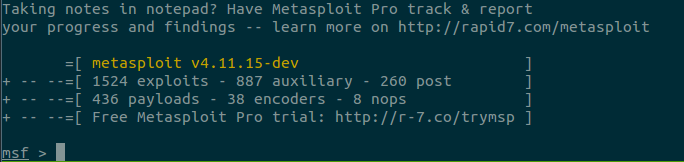
\includegraphics[width=\textwidth]{images/msfconsole.png}
            \caption{Lancement de Metasploit}
            \label{msfconsole}
        \end{subfigure}
        \hfill
        \begin{subfigure}{0.9\textwidth}
            \centering
            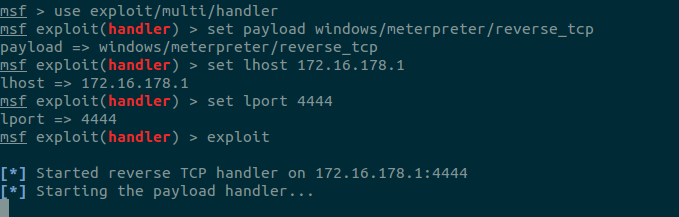
\includegraphics[width=\textwidth]{images/ecoute_msf.png}
            \caption{Configuration de Metasploit}
            \label{config_metasploit}
        \end{subfigure}
        \hfill
        \caption{Préparation de Metasploit}
        \label{prepration_metasploit}
    \end{figure}

    Maintenant, il ne reste plus qu'à lancer le script d'exploitation que nous avons modifié et obtenir un accès à la 
    machine exploitée (\autoref{obtention_accees_meterpreter}).

    \begin{figure}[H]
        \centering
        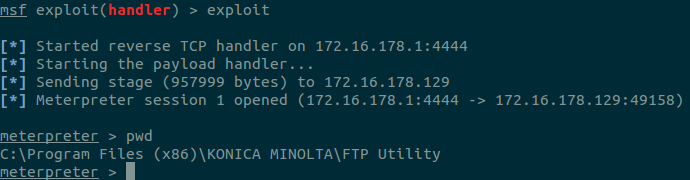
\includegraphics[width=\linewidth]{images/meterpreter.png}
        \caption{Obtention de l'accès avec meterpreter}
        \label{obtention_accees_meterpreter}
    \end{figure}

\section{Teste de propagation}
Cette partie contiendra une simulation de propagation du Malware développé au cours de ce projet et 
l'infection d'une machine sécurisée.

Pour cela, nous procédons au test sur l’environnement cité auparavant dans la \autoref{preparation_environnement}.

Tout d'abord, nous infectons un exécutable quelconque de notre clé USB, cela encapsulera le corps du virus et du 
backdoor dedans. Puis nous exploitons la vulnérabilité présente dans la machine de faible sécurité pour avoir 
accès au Shell de cette dernière (comme expliqué dans la \autoref{exploitation}), de ce fait, nous envoyons 
l'exécutable préparé puis nous l’exécutons (\autoref{launch_virus})

\begin{figure}[H]
    \centering
    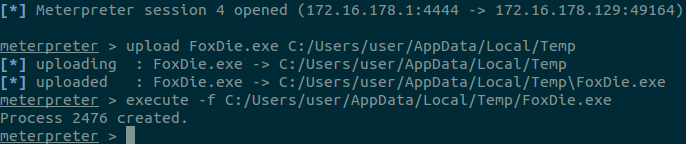
\includegraphics[width=\linewidth]{images/exec_virus.png}
    \caption{Envoi et exécution du virus}
    \label{launch_virus}
\end{figure}
Cela infectera la machine et tout fichier exécutable contenu dans des périphériques de stockage externe qui sont, ou qui vont  être connectés à cette machine.  Nous pouvons constater que le processus de notre Virus est en exécution sur la machine, et nous pouvons aussi observer qu'à chaque minute, le backdoor est exécuté (\autoref{process_backdoor}).

\begin{figure}[H]
    \centering
    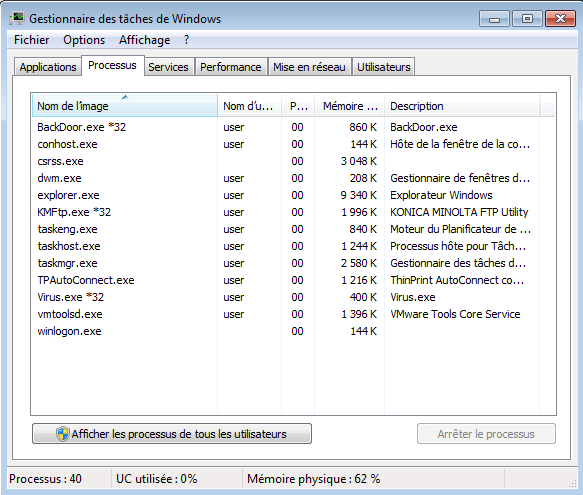
\includegraphics[width=\linewidth]{images/processus_backdoor.png}
    \caption{Processus du backdoor}
    \label{process_backdoor}
\end{figure}

Pour la deuxième étape de notre test, nous connectons une clé usb contenant plusieurs fichiers, dont des exécutables et autres (\autoref{avant_infection}). À ce titre, nous pouvons constater que la taille des exécutables s'agrandit de 144 Ko (\autoref{apres_infection}), cela veut dire que les deux segments (le virus et le backdoor) ont été ajoutés correctement.

\begin{figure}[H]
    \centering
    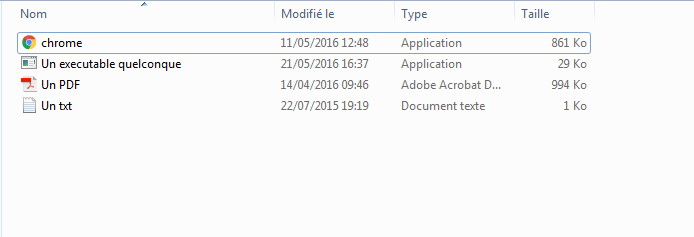
\includegraphics[width=\linewidth]{images/avant_infeciton.png}
    \caption{Avant Infection}
    \label{avant_infection}
\end{figure}

\begin{figure}[H]
    \centering
    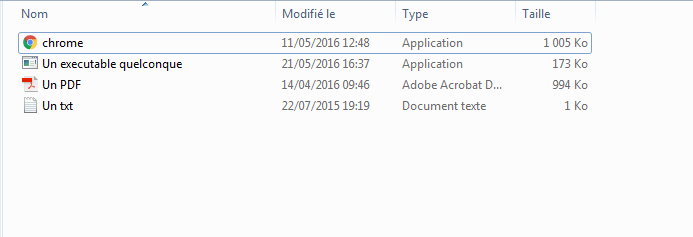
\includegraphics[width=\linewidth]{images/apres_infection.png}
    \caption{Après Infection}
    \label{apres_infection}
\end{figure}

Nous prenons cette clé, puis nous la connectons à la machine qui est hautement sécurisée. Nous essayons de 
l'analyser avec le fameux Anti Virus \emph{Kaspersky} qui après analyse indique que tous les fichiers contenus 
dans la clé sont sains et non infectés (\autoref{scan_cle}). Nous procédons alors à l’exécution de l'un des 
fichiers exécutables comme le ferait n'importe quel usager utilisant un Anti Virus.

\begin{figure}[H]
    \centering
    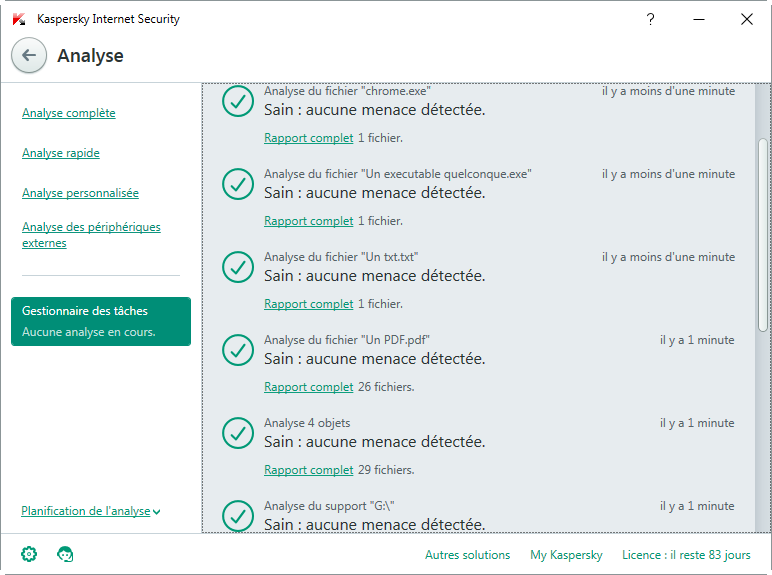
\includegraphics[width=\linewidth]{images/scan_by_antivirus.png}
    \caption{Scan de la clé USB}
    \label{scan_cle}
\end{figure}

À cet effet, le code malveillant contenu dans le logiciel infecté s’exécute en premier comme cité dans la 
\autoref{virus_infecteur}, et fera la tâche qui lui a été assignée.

Par la suite, nous lançons notre serveur dans notre machine en écoute et nous attendons que le backdoor qui 
s'exécute dans la machine sécurisée se connecte vers ce dernier. Après un délai, la connexion s'effectue 
(\autoref{connect_backdoor}), ce qui nous donne finalement un accès total à la machine réputée comme étant protégée.

\begin{figure}[H]
    \centering
    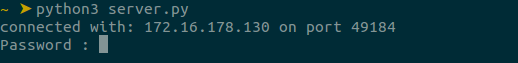
\includegraphics[width=\linewidth]{images/backdoor_connect.png}
    \caption{Connexion du backdoor à notre serveur}
    \label{connect_backdoor}
\end{figure}

\section{Conclusion}
À la fin du chapitre final, nous avons réussi à développé un Malware hybride. Ce Malware a prouvé son efficacité
contre les anti-virus, et il a réussi à atteindre la machine sécurisée par le biais d'une propagation furtif.
